% =====================================================================
% AI Academy -- National AI Center
% Software Engineering Final Project -- Team Presentation Deck
%
% Built from templates/SLIDES_TEMPLATE.tex (preamble and slide order kept).
% Changes to the template: a fourth member, the EVIDENCE VALUES block, a
% graphics path for the shared architecture figure, a shell listing style,
% a full-width footer (the original footer text ran together), and one extra
% content slide for the cache evidence.
%
% Compile with pdfLaTeX twice (Overleaf: upload this file together with
% docs/figures/architecture.pdf). Do not commit .aux/.log/.nav/.out/.snm/.toc.
% =====================================================================

\PassOptionsToPackage{dvipsnames}{xcolor}
\documentclass[aspectratio=169,11pt]{beamer}

% ===== CONFIGURATION ==================================================
\newcommand{\teamname}{Research Assistant Team}
\newcommand{\topicchoice}{Topic 4 -- Async Research Assistant}
\newcommand{\memberone}{Ruslan Sadigov}
\newcommand{\membertwo}{Nihat Ismayilzade}
\newcommand{\memberthree}{Samur Eyyubov}
\newcommand{\memberfour}{Polad Ibrahimli}
\newcommand{\repolink}{github.com/ruslan-sadigov/research-assistant-SWE-Final-Project}
\def\defensedate{} % set when known, e.g. \def\defensedate{24 September 2026}

\newcommand{\coursecode}{AI-ENG-110}
\newcommand{\coursename}{Software Engineering}
\newcommand{\institution}{AI Academy, National AI Center}
\newcommand{\semester}{Spring 2026}

% ===== EVIDENCE VALUES ================================================
% Must equal the final report. Sources: pytest/coverage run of the branch,
% docs/docker.md, and git shortlog on main (author aliases merged).
\newcommand{\owntests}{267}
\newcommand{\smoketests}{16}
\newcommand{\coveragepct}{98.44}
\newcommand{\imagesize}{218.67\,MB}
\newcommand{\commitdate}{18 Sep 2026}
\newcommand{\committotal}{81}
\newcommand{\commitsone}{53 (65.4\%)}
\newcommand{\commitstwo}{6 (7.4\%)}
\newcommand{\commitsthree}{12 (14.8\%)}
\newcommand{\commitsfour}{10 (12.3\%)}

% ===== PACKAGES ======================================================
\usepackage[T1]{fontenc}
\usepackage[utf8]{inputenc}
\usepackage{xcolor}
\usepackage{tabularx}
\usepackage{booktabs}
\usepackage{listings}
\usepackage{tikz}
\usetikzlibrary{shapes.geometric,arrows.meta,positioning,fit,backgrounds}
\graphicspath{{../docs/figures/}{./}}

% ===== EARLY MACROS ==================================================
\definecolor{accent2}{HTML}{8B0000}
\newcommand{\TODO}[1]{\textcolor{accent2}{\textbf{[TODO: #1]}}}

% ===== BEAMER THEME (custom, no flashy decorations) =================
\usetheme{default}
\usefonttheme{professionalfonts}
\setbeamertemplate{navigation symbols}{}

\definecolor{accent}{HTML}{0B3D91}
\definecolor{soft}{HTML}{F2F4F8}
\definecolor{ok}{HTML}{166534}

\setbeamercolor{title}{fg=accent}
\setbeamercolor{frametitle}{fg=accent}
\setbeamercolor{section in head/foot}{bg=accent,fg=white}
\setbeamercolor{itemize item}{fg=accent}
\setbeamercolor{itemize subitem}{fg=accent}
\setbeamercolor{enumerate item}{fg=accent}
\setbeamercolor{block title}{bg=accent,fg=white}
\setbeamercolor{block body}{bg=soft,fg=black}

\setbeamerfont{title}{size=\Large,series=\bfseries}
\setbeamerfont{frametitle}{size=\large,series=\bfseries}
\setbeamerfont{footline}{size=\tiny}

% Footer with team + slide number
\setbeamertemplate{footline}{%
  \leavevmode%
  \hbox to \paperwidth{\hspace*{2ex}\tiny\textit{\teamname{} -- \topicchoice}\hfill%
  \tiny\textit{\coursecode{} -- \semester{}}\hfill%
  \tiny\insertframenumber/\inserttotalframenumber\hspace*{2ex}}%
  \vskip1pt%
}

% ===== CODE LISTINGS =================================================
\definecolor{codegreen}{rgb}{0,0.55,0}
\definecolor{codepurple}{rgb}{0.55,0,0.78}
\lstdefinestyle{python}{
  language=Python,
  backgroundcolor=\color{soft},
  commentstyle=\color{codegreen},
  keywordstyle=\color{accent},
  stringstyle=\color{codepurple},
  basicstyle=\ttfamily\scriptsize,
  breaklines=true,
  frame=single,
  framerule=0.4pt,
  rulecolor=\color{black!30},
}
\lstdefinestyle{shell}{
  basicstyle=\ttfamily\scriptsize,
  upquote=true,
  backgroundcolor=\color{soft},
  columns=fullflexible,
  keepspaces=true,
  frame=single,
  framerule=0.4pt,
  rulecolor=\color{black!30},
}

% =====================================================================
\begin{document}

% ========== SLIDE 1: TITLE ===========================================
{%
\setbeamertemplate{footline}{}
\begin{frame}[plain]
  \begin{center}
    \vspace{0.6cm}
    {\small \textsc{\institution}}\\[0.2em]
    {\small \textsc{\coursecode{} -- \coursename{} -- \semester{}}}\\[1.2em]
    \rule{0.7\textwidth}{0.6pt}\\[0.4em]
    {\LARGE\bfseries\color{accent} \topicchoice}\\[0.4em]
    \rule{0.7\textwidth}{0.6pt}\\[1.2em]
    {\large \teamname}\\[0.6em]
    {\normalsize \memberone\quad\textbullet\quad\membertwo\quad\textbullet\quad\memberthree\quad\textbullet\quad\memberfour}\\[1cm]
    {\footnotesize\itshape Final Project Defense\ifx\defensedate\empty\else{} -- \defensedate\fi}\\[0.4em]
    {\footnotesize\texttt{\repolink}}
  \end{center}
\end{frame}
}

% ========== SLIDE 2: PROBLEM =========================================
\begin{frame}{The problem in one sentence}
  \begin{block}{What the system does}
    A user asks a research question; the tool collects evidence from Wikipedia, arXiv and
    web search at the same time and prints an LLM answer whose numbered citations point to
    that evidence. A failing source becomes a warning, not a crash.
  \end{block}

  \vspace{0.3em}
  \begin{columns}[T,onlytextwidth]
  \column{0.48\textwidth}
  \textbf{Inputs}
  \begin{itemize}
    \item Question text, up to 2000 characters
    \item Sources: any of \texttt{wiki}, \texttt{arxiv}, \texttt{web}
    \item Optional \texttt{-{}-no-cache}; keys and limits from \texttt{.env}
  \end{itemize}

  \column{0.48\textwidth}
  \textbf{Outputs}
  \begin{itemize}
    \item Answer, references, per-source warnings
    \item Exit code 0 (answer), 1 (none), 2 (invalid input)
    \item Source evidence cached in SQLite for 24\,h
  \end{itemize}
  \end{columns}

  \vspace{0.4em}
  \textbf{Entry point:} CLI only, no HTTP server:\enspace
  {\small\texttt{python -m researcher ask "..." -{}-sources wiki,arxiv,web}}
\end{frame}

% ========== SLIDE 3: ARCHITECTURE ====================================
\begin{frame}{Architecture}
  \textbf{Module map.} The boundary between the \emph{provided} \texttt{ai/} package
  (red, dashed) and \emph{our} SE layer is shown explicitly.

  \vspace{0.2em}
  \begin{center}
  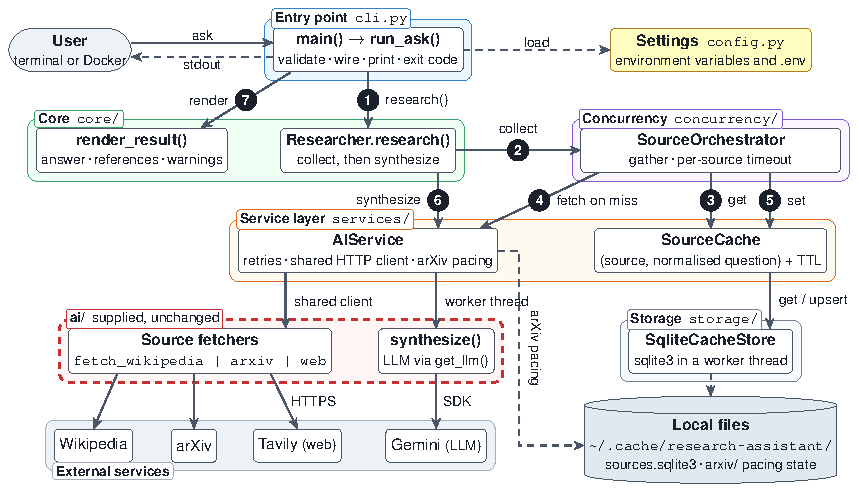
\includegraphics[width=\textwidth,height=0.72\textheight,keepaspectratio]{architecture.pdf}
  \end{center}
  \vspace{-0.6em}
  {\scriptsize Solid arrows: calls, numbered in request order. Dashed: configuration, local files, output.}
\end{frame}

% ========== SLIDE 4: TECHNOLOGY STACK ================================
\begin{frame}{Technology stack}
  \begin{center}\scriptsize
  \begin{tabularx}{\linewidth}{@{}>{\raggedright\arraybackslash}p{0.17\linewidth}>{\raggedright\arraybackslash}p{0.36\linewidth}X@{}}
    \toprule
    \textbf{Layer} & \textbf{Technology} & \textbf{Why this one} \\
    \midrule
    Language, runtime & Python 3.12, \texttt{asyncio} & \texttt{gather}, \texttt{timeout} and \texttt{to\_thread} are in the standard library \\
    Environment & \texttt{uv} with a locked \texttt{uv.lock} & Same versions locally, in CI and in Docker \\
    Config, models & \texttt{pydantic-settings}, \texttt{python-dotenv}, Pydantic v2 & Typed settings and self-validating boundary types \\
    HTTP & \texttt{httpx} async client + our \texttt{RetryingTransport} & One shared client; retries and pacing in one place \\
    Storage & SQLite (standard \texttt{sqlite3}) & No server to run; the file survives restarts in a volume \\
    Providers (in \texttt{ai/}) & Wikipedia, arXiv, Tavily, Gemini & Supplied package; chosen by environment variables \\
    Tests & \texttt{pytest}, \texttt{pytest-asyncio}, \texttt{pytest-cov}, \texttt{MockTransport} & Async tests, offline, with coverage \\
    Quality gates & Ruff, Black, isort, mypy & One style and typed signatures across four authors \\
    Delivery & GitHub Actions, multi-stage Docker & Lint, types, tests and an image on every push \\
    \bottomrule
  \end{tabularx}
  \end{center}

  \vspace{0.3em}
  {\footnotesize Everything except the \texttt{ai/} package and its providers is our own code and configuration.}
\end{frame}

% ========== SLIDE 5: KEY DESIGN DECISIONS ============================
\begin{frame}{Three design decisions we can defend}
  \begin{enumerate}\setlength\itemsep{0.5em}
    \item \textbf{asyncio over threads, one deadline per source}\\
      All work is waiting on at most three sources, so one event loop is enough.
      Rejected: threads, and \texttt{TaskGroup}, which cancels the other sources when one fails.
    \item \textbf{Protocols and constructor injection around the unchanged \texttt{ai/}}\\
      Tests swap in fakes without patching. Trade-off accepted: one wiring function
      (\texttt{run\_ask}) must build everything in the right order.
    \item \textbf{SQLite cache of source evidence, not of answers}\\
      Every run still synthesizes; repeated questions skip the network. We would change it
      for many parallel users (single-file writer) or if answers became expensive.
  \end{enumerate}

  \vspace{0.5em}
  \begin{block}{Expect to be asked}
    ``Why did you not use threads / a semaphore / Redis / an answer cache?''
    Have a 15-second answer ready for each of the three.
  \end{block}
\end{frame}

% ========== SLIDE 6: CONCURRENCY (THE BENCHMARK) =====================
\begin{frame}{Concurrency: the benchmark}
  \textbf{Workload:} the 5 supplied questions $\times$ all 3 sources, cache off.
  Offline: simulated delays 0.1\,/\,0.2\,/\,0.3\,s, median of 5 runs.
  Live: Wikipedia, arXiv, Tavily, one pair per question.

  \vspace{0.3em}
  \begin{center}\small
  \begin{tabular}{lcc}
    \toprule
    & \textbf{Sequential} & \textbf{Concurrent (gather, $\le$3 tasks)} \\
    \midrule
    Offline wall-clock (s) & 0.623--0.628 & 0.312--0.314 \\
    Offline speedup        & 1.0$\times$  & 1.99--2.00$\times$ \\
    Live wall-clock (s)    & 4.41--7.04   & 3.62--5.60 \\
    Live speedup (q1--q5)  & 1.0$\times$  & 0.79--1.82$\times$ \\
    Failed or timed-out sources & 0 & 0 \\
    \bottomrule
  \end{tabular}
  \end{center}

  \vspace{0.3em}
  \textbf{Bottleneck named:} the slowest source sets the concurrent time (0.3\,s offline);
  live, network latency and arXiv's 3\,s request spacing.\\
  \textbf{What didn't reach $N\times$:} with unequal delays the ideal is 2$\times$, not 3$\times$;
  live, q2 was slower concurrently and Wikipedia found nothing for full questions.

  \vspace{0.2em}
  {\footnotesize\textit{Reproduce (README):} \texttt{uv run python benchmarks/benchmark\_sources.py -{}-repeats 5}}
\end{frame}

% ========== SLIDE 7: ROBUSTNESS STORY ================================
\begin{frame}{Robustness: one concrete failure mode}
  \textbf{Scenario:} in a live run with all three sources, arXiv timed out.

  \vspace{0.3em}
  \textbf{How we surfaced it:} manual live CLI run; reproduced offline in
  \texttt{test\_deadline\_cancels\_slow\_fetch\_and\_preserves\_success}.

  \vspace{0.3em}
  \textbf{What the system does:}
  \begin{itemize}\setlength\itemsep{0.25em}
    \item \textbf{Retry:} up to 3 attempts, 0.5\,s growing to 4\,s, only for timeouts, 408, 429
      and 5xx; \texttt{Retry-After} honoured; one 10\,s deadline per source.
    \item \textbf{Validate:} input and settings checked before any call (exit 2);
      models reject unknown fields; cached rows re-validated on read.
    \item \textbf{Log:} \texttt{source timeout: source=arxiv stage=... deadline\_expired=...};
      failures log the error type only, no keys or messages.
    \item \textbf{Degrade:} Wikipedia's evidence was kept and the answer was printed with an
      arXiv warning; exit code 0.
  \end{itemize}

  \vspace{0.2em}
  {\footnotesize Also seen live: intermittent Gemini 503 (high demand); later calls succeeded.}
\end{frame}

% ========== SLIDE 8: CACHE EVIDENCE (added) ==========================
\begin{frame}{Caching: measured, not assumed}
  \begin{columns}[T,onlytextwidth]
  \column{0.52\textwidth}
  \textbf{Schema and policy}
  \begin{itemize}\setlength\itemsep{0.2em}
    \item Table \texttt{cache\_entries}: key \texttt{(source, query\_key)}, its automatic
      unique index, JSON \texttt{payload}; no foreign keys
    \item Key = source + normalised question; TTL 24\,h
    \item All rows derived; the external sources stay authoritative
    \item \texttt{-{}-no-cache} never opens the SQLite file
  \end{itemize}

  \column{0.44\textwidth}
  \textbf{Hit rate} = hits / lookups
  \begin{center}\small
  \begin{tabular}{lr}
    \toprule
    First run  & 0 / 15 \\
    Second run & 15 / 15 \\
    \textbf{Combined} & \textbf{15 / 30 = 50\%} \\
    \bottomrule
  \end{tabular}
  \end{center}
  {\footnotesize 5 questions $\times$ 3 sources through the real CLI; providers simulated;
  an answer synthesized on every run.}
  \end{columns}

  \vspace{0.4em}
  \textbf{Staleness:} empty results are also kept for 24\,h, and the key ignores provider settings.

  \vspace{0.2em}
  {\footnotesize\textit{Reproduce:} \texttt{uv run python tests/cache\_verification.py}
  \enspace\textit{(docs/cache-verification.md)}}
\end{frame}

% ========== SLIDE 9: DEMO ============================================
\begin{frame}[fragile]{Live demo (or scripted demo)}
  \begin{block}{What we will run}
    One question against all three sources, twice, with a cache volume: the second run is
    served from SQLite and still produces an answer.
  \end{block}

  \vspace{0.2em}
  \textbf{Demo command (works inside Docker):}
\begin{lstlisting}[style=shell]
docker run --rm --env-file .env --env DATABASE_URL= `
  -v research-assistant-cache:/home/appuser/.cache/research-assistant `
  research-assistant:runtime ask "Photovoltaic effect" --sources wiki,arxiv,web
\end{lstlisting}

  \begin{itemize}\setlength\itemsep{0.15em}
    \item On screen: numbered references from all three sources; on the second run,
      \texttt{cache\_hit=True} in the log.
    \item Timing: in a live container run the sources took 2.39, 3.53 and 0.53\,s, yet
      collection finished in 3.64\,s instead of 6.45\,s.
  \end{itemize}

  \vspace{0.1em}
  {\footnotesize\textit{Backup: pre-recorded screencast, then the offline run
  \texttt{uv run python tests/cache\_verification.py}.}}
\end{frame}

% ========== SLIDE 10: TESTING =========================================
\begin{frame}{Testing}
  \begin{columns}[T,onlytextwidth]
  \column{0.44\textwidth}
  \textbf{Coverage \& shape}
  \begin{itemize}\setlength\itemsep{0.3em}
    \item Total coverage: \coveragepct\,\%
    \item Provided \texttt{ai/} smoke tests: \textcolor{ok}{\textbf{passing}}
    \item Test count: \owntests{} own + \smoketests{} smoke
    \item All tests offline; AI module fully mocked
  \end{itemize}

  \column{0.53\textwidth}
  \textbf{Three tests worth calling out}
  \begin{itemize}\setlength\itemsep{0.3em}
    \item \textbf{Happy path:} the real CLI answers each supplied question, reuses SQLite,
      then honours \texttt{-{}-no-cache}.
    \item \textbf{Concurrency:} arXiv raises, gather degrades; Wikipedia and web evidence kept.
    \item \textbf{Error path:} HTTP 408/429/500/503 is retried once, then succeeds;
      every response is closed.
  \end{itemize}
  \end{columns}

  \vspace{0.6em}
  \begin{block}{Tooling}
    \texttt{pytest} + \texttt{pytest-asyncio} + \texttt{pytest-cov} + \texttt{httpx.MockTransport}.
    mypy: no issues in 15 source files; Ruff, Black and isort clean in CI.
  \end{block}
\end{frame}

% ========== SLIDE 11: LIMITATIONS + FUTURE ===========================
\begin{frame}{Limitations \& what we'd do next}
  \textbf{Where the system is brittle today}
  \begin{itemize}\setlength\itemsep{0.3em}
    \item Full questions often find no Wikipedia match; there is no query rewriting.
    \item No fallback LLM: if Gemini is down, we show evidence but no answer.
    \item The cache keeps empty results for 24\,h, ignores provider settings, and never evicts rows.
  \end{itemize}

  \vspace{0.4em}
  \textbf{Given another week we would}
  \begin{enumerate}\setlength\itemsep{0.3em}
    \item Turn the question into a short topic query before searching Wikipedia.
    \item Add a settings fingerprint to the cache key, a shorter TTL for empty results, and a purge command.
    \item Repeat the live benchmark at least three times and compare distributions.
  \end{enumerate}
\end{frame}

% ========== SLIDE 12: TEAM CONTRIBUTIONS =============================
\begin{frame}{Team contributions}
  \begin{center}\footnotesize
  \begin{tabularx}{\linewidth}{lXl}
    \toprule
    \textbf{Member} & \textbf{Primary ownership} & \textbf{Commits} \\
    \midrule
    \memberone   & Settings, models, interfaces, orchestrator, retry transport, arXiv pacing; merges and release & \commitsone \\
    \membertwo   & AIService around \texttt{ai/}; engineering audit, tests, Docker and provider docs & \commitstwo \\
    \memberthree & SourceCache and SQLite store; architecture diagram, cache verification, slides, demo & \commitsthree \\
    \memberfour  & CLI and Researcher; report, README, contribution statement & \commitsfour \\
    \bottomrule
  \end{tabularx}
  \end{center}
  \vspace{-0.4em}
  {\scriptsize Commits on \texttt{main}, \commitdate{}, \committotal{} in total, author aliases merged.
  Final shares: signed contribution statement.}

  \vspace{0.4em}
  \begin{block}{We can all answer:}
    Any of us can walk through any module on demand. Pick a file --- we'll defend it.
  \end{block}

  \vspace{0.3em}
  {\small\textbf{AI tool use:} disclosed per member in the contribution statement; e.g.\ Claude
  drafted Samur's architecture figure, cache tests and this deck, which Samur reviewed and ran.}
\end{frame}

% ========== SLIDE 13: THANK YOU / Q&A ================================
{%
\setbeamertemplate{footline}{}
\begin{frame}[plain]
  \begin{center}
    \vspace{1cm}
    {\Huge\bfseries\color{accent} Questions?}\\[1.2em]
    \rule{0.5\textwidth}{0.6pt}\\[1.2em]
    {\large \teamname}\\[0.6em]
    {\small \texttt{\repolink}}\\[1cm]
    {\footnotesize\itshape ``We can walk through any file in the repo.''}
  \end{center}
\end{frame}
}

\end{document}
